% @file documentary.tex
% @project IAL Náhradní projekt - 05. Rovinnost grafu
% @author Vladimir Meciar (xmecia00)
% @brief This file includes documentation of project
% @note Lots of work was reused from documentation in https://gitlab.com/TheRealTom/IFJ21.
%       Docuentation in IFJ21 project was my work (revision be teamates)
% @changes 7.12.2022

% Preamble
\documentclass[12pt,a4paper]{article}

% Packages
\usepackage[czech]{babel}
\usepackage[utf8]{inputenc}
\usepackage[T1]{fontenc}
\usepackage{float}
\usepackage{lmodern}
\usepackage[none]{hyphenat}
\usepackage[left=2cm, text={17cm, 24cm}, top=2cm]{geometry}
\usepackage{graphicx}
\usepackage{xcolor}
\usepackage{amsmath}
\usepackage{amssymb}
\usepackage{caption}
\usepackage{subcaption}
\usepackage{titlesec}
\usepackage{hyperref}
\usepackage{listings}
\usepackage{enumitem}
\usepackage{wasysym}
\usepackage{fancyhdr}
\usepackage{lastpage}
\usepackage{newpxtext}
\usepackage{longtable,ltcaption}
\usepackage{textgreek}
\usepackage{multirow}

\newcommand{\comment}[1]{}


% Document
\begin{document}

    % Front page
    \pagestyle{empty}
    \begin{titlepage}
        \begin{center}
            \normalsize{Vysoké učení technické v Brně\linebreak}
            \normalsize{Fakulta informačních technologií}

            \vfill

            \large\textbf{Algoritmy\linebreak Rovinnost grafu}
            \large\textbf{2022/2023}

            \vfill

            \LARGE\textbf{Technická zpráva\linebreak}

            \vfill
            \vfill
            \vfill


            \begin{flushleft}
                \large
                \textbf{Rastislav Mazúr  (xmazur09)}\\
                Jakub Kavka (xkavka02)\\
                Ondřej Podroužek (xpodro03)\\
                Vladimír Mečiar (xmecia00)\\
                \hfill

                Brno, \today
            \end{flushleft}
        \end{center}
    \end{titlepage}
    \pagestyle{plain}
    \newpage

    % Content - sections
    \tableofcontents
    \newpage

    % Conent - pictures and tables
    % \listoffigures
    % \listoftables
    % \newpage

    % Content
    % @file zadanie.tex
% @project IAL Náhradní projekt - 05. Rovinnost grafu
% @author Vladimir Meciar (xmecia00)
% @brief This file id module for documentation.tex with specified task
% @changes 7.12.2022
\section{Zadání varianty}
Graf je rovinný, jestliže lze jeho vrcholy (jako body) a hrany (jako spojité křivky) umístit do roviny tak, aby se žádné dvě hrany nekřížily.\\


Vytvořte program, který rozhodne, zda je graf rovinný.\\
Součástí projektu bude načítání grafů ze souboru a vhodné testovací grafy. V dokumentaci uveďte teoretickou složitost úlohy a porovnejte ji s experimentálními výsledky. Nepředpokládá se, že by nalezení rozmístění vrcholů a hran v rovině bylo součástí řešení.
Pozor! Otestování rovinnosti grafu je netriviální problém. Můžete použít algoritmus založený na tvrzení pana Kuratowského (1930): Rovinný graf neobsahuje podgraf izomorfní s grafy K(5) nebo K(3,3).
    % @file documentary.tex
% @project IAL Náhradní projekt - 05. Rovinnost grafu
% @author Vladimir Meciar (xmecia00)
% @brief This file id module for documentation.tex describeing work in team
% @changes 7.12.2022
\section{Práce v týmu}

\subsection{Rozdělení práce}
První s schůzku jsme měli v oktobri.
Touto dobou jsme se seznamovali a začali sme rozoberat zakladnu problematiku grafov. Sucastou bolo aj urcenie algoritmu
na odhalenie planarity grafu.
Od tejto casti sme nanestasie dlho nijako nepokrocili nakolko sme mali na starosti ine poinnosti suvisiace so skolou

Práci jsme neměli dopředu rezdělenou a úkoly jsme si rozdělovali podle potřeby v průběhu práce.

\begin{enumerate}
    \item[] Navrh a implementacia automatu pre prijmanie znakov
    \begin{itemize}[noitemsep,topsep=0pt]
        \item Ondrej Podrouzek
    \end{itemize}

    \item[] Testovanie automatu
    \begin{itemize}[noitemsep,topsep=0pt]
        \item Rastislav Mazur
    \end{itemize}

    \item[] Navrh, implementacia a testovanie datovej struktury pre ukladanie grafu
    \begin{itemize}[noitemsep,topsep=0pt]
        \item Vladimír Mečiar
    \end{itemize}


    \item[] Implementacia finalnej logiky programu
    \begin{itemize}[noitemsep,topsep=0pt]
        \item Jakub Kavka
    \end{itemize}

    \item[] Testovanie finalnej logiky programu
    \begin{itemize}[noitemsep,topsep=0pt]
        \item Rastislav Mazur
    \end{itemize}


    \item[] Tvorba dokumentace
    \begin{itemize}[noitemsep,topsep=0pt]
        \item Vladimír Mečiar
    \end{itemize}

    \item[] Revizia kodu a dokumentacie
    \begin{itemize}[noitemsep,topsep=0pt]
        \item Rastislav Mazur, Ondrej Podrouzek
    \end{itemize}

\end{enumerate}


\subsection{Verzování}
Pro sdílení a verzování kódu jsme použili verzovací systém GitHub.

V projektu jsme pracovali na více částech současně.
Pro každou větší část jsme vytvářeli vlastní větve, které jsme po dokončení mergovali do větve \texttt{develop}.
Do finální verze repozitara \texttt{main} jsme prepojili až finální otestovanou verzi a následně jsme přímo v ní prováděli jen poslední úpravy.

\subsection{Komunikace}
Jako komunikační platformy jsme využili \textit{Discord}, který sloužil jako hlavní komunikační kanál.
Pro sdílení učebních materiálů jsme vytvořili \texttt{Discord} server.
    % @file conlusion.tex
% @project IAL Náhradní projekt - 05. Rovinnost grafu
% @author Vladimir Meciar (xmecia00)
% @brief This file is module for documentation.tex with documantation for scanner
% @changes 7.12.2022
\section{Nacitanie dat}
    % @file conlusion.tex
% @project IAL Náhradní projekt - 05. Rovinnost grafu
% @author Vladimir Meciar (xmecia00)
% @brief This file is module for documentation.tex with documentation for data structure
% @changes 7.12.2022
\section{Ukladanie dat}

\section{Datova struktura}

Pre ulozenie dat sme si potrebovali vybrat vhodnu datovu strukturu. V nasom pripade sme pouzili nafukovacie pole.
Nadedinovali sme si ju ako strukturu s nazvom vektor. Potom nam zostalo uz len ulozit uzly.Pre tie sme si nadefinovali zvlast strukturu

\begin{figure}[h]
    \centering
    \begin{subfigure}[b]{0.3\textwidth}
        \centering
        
\includegraphics[width=\textwidth]{doc/fig/vector.png}
        \caption{Vektor}
        \label{fig:vector}
    \end{subfigure}
    \hfill
    \begin{subfigure}[b]{0.3\textwidth}
        \centering
        
\includegraphics[width=\textwidth]{doc/fig/graph.png}
        \caption{Graf}
        \label{fig:graph}
    \end{subfigure}
    \hfill
    \begin{subfigure}[b]{0.3\textwidth}
        \centering
        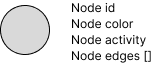
\includegraphics[width=\textwidth]{doc/fig/node.png}
        \caption{Uzol}
        \label{fig:five over x}
    \end{subfigure}
    \caption{Three simple graphs}
    \label{fig:three graphs}
\end{figure}



    % @file conlusion.tex
% @project IAL Náhradní projekt - 05. Rovinnost grafu
% @author Vladimir Meciar (xmecia00)
% @brief This file is module for documentation.tex with final logic for program
% @changes 7.12.2022
\section{Finalna logika}
    % @file testing.tex
% @project IAL Náhradní projekt - 05. Rovinnost grafu
% @author Vladimir Meciar (xmecia00)
% @brief This file is module for documentation.tex with specification of workflow for test
% @changes 7.12.2022
\section{Testovanie}

Na testovanie sme pouzili porovnanie aktualnych vysledkov programu s referencnymi vysledkami.
Rozdelenie bolo pouzite ako v pribalenom Makefile.

\begin{itemize}
    \item Testovanie datovych struktur
    \item Testovanie Lexikalneho analyzatoru
    \item Testovanie finalnej logiky algpritmu
\end{itemize}

Napomocne nam boli skripty v adresari test
    % @file conlusion.tex
% @project IAL Náhradní projekt - 05. Rovinnost grafu
% @author Vladimir Meciar (xmecia00)
% @brief This file is module for documentation.tex with conclusion
% @changes 7.12.2022
\section{Závěr}
Při řešení jsme narazili na spousta nejasností, které jsme museli řešit na Discordu, nebo některá na fóru projektu.

Celkově byl tento projekt přínosný. Naučili jsme se práci v týmu a organizování času.
Velkým přínosem byly zejména zkušenosti s verzovacími systémy \textit{Git}.

\newpage

\end{document}
